\documentclass{article}
\usepackage[utf8]{inputenc}
\usepackage[italian]{babel}
\usepackage[a4paper, total={6in, 10in}]{geometry}
\usepackage{hyperref}
\usepackage{float}
\usepackage{graphicx}
\graphicspath{ {./img/} }

\title{ \textbf{Relazione ingegneria - Progetto Monopoly}}
\author {\textbf{Team Gang of Four 2}\\Acerbis Gianluca\\Canesi Gabriele\\Di Pierro Luca\\Fiorenza Gioele}
\date{\today}

\begin{document}

\maketitle

\section{Analisi}

\subsection{Premessa}
Essendo alcuni diagrammi particolarmente grandi, abbiamo preferito, per poter permettere la loro visione  renderli consultabili attraverso il browser.
Cliccando sulle immagini si verrà di fatto portati al diagramma relativo, laddove quest'ultimo sia ritenuto troppo grande per essere consultato dal documento pdf.

\subsection{Requisiti extra richiesti dal progetto}
Qui sotto descriviamo come abbiamo interpretato le richieste ulteriori mosse per il progetto:
\begin{itemize}
	\item \textbf{Random sequence of sposts, periodic random change of proprerty pricing, rents e interest e tax rates (both in sposts and cards)}: 
		Questo punto è abbastanza chiaro e abbiamo implementato tutto ciò che era richiesto (cambi random di sequenza caselle, cambi nei prezzi di caselle proprietà e tasse nonché cambiamenti per le carte imprevisti e probabilità).
	Questo avviene solo se la difficoltà del gioco è impostata su difficile.
	
	\item \textbf{Allow new player to join the game as enterpreneurs}: 
		In questo caso diamo la possibilità, in base alla difficoltà del gioco (normale o difficile), agli utenti di entrare come imprenditori. Gli imprenditori pagano il 5\% in meno sugli affitti ma tasse del 75\% più elevate.
	Percentuale calcolata in base al rateo proprietà/tasse che sono presenti sul terreno.
	
	\item \textbf{Allow complexity setting in three levels (easy, medium, hard)}: 
		Abbiamo suddiviso le difficoltà come segue:
		\begin{itemize}
			\item \textbf{Easy}: gioco vanilla senza aggiunte
			\item \textbf{Medium}: è possibile entrare come Imprenditore in partita
			\item \textbf{Hard}: Tabellone randomizzato, cambi tassi periodici per Caselle(proprietà \& tasse) e Imprevisti\&Probabilità	
		\end{itemize}
		
	\item \textbf{Allow a loyalty program to enable the use of virtual currency with random rules based on existing international alliances' programs}: 
		Non siamo stati in grado di comprendere in alcun modo come fosse possibile integrare un loyalty program collegato a alleanze internazionali(?) in monopoly.
	Inoltre si parla di virtual currency (cosa che è già presente di base di base nel gioco)
		
\end{itemize}	

\subsection{Documenti Prodotti}
	
\subsubsection{Caso D'Uso UC1: Gioca Turno}
\begin{enumerate}
    \item Il giocatore lancia i dadi
    \item La pedina del giocatore avanza del numero indicato dalla somma dei dadi.
\end{enumerate}
\subsection{Scenari alternativi}
\begin{enumerate}
    \item [1a] Il giocatore si trova in prigione e non sono ancora passati 3 turni dall'ultimo lancio:
    \begin{enumerate}
        \item il caso d'uso termina
    \end{enumerate}
    \item [1b] Il giocatore si trova in prigione e sono passati 3 turni dall'ultimo lancio:
        \begin{enumerate}
            \item Il giocatore lancia i dadi
            \item Se i dadi hanno valore uguale, il giocatore esce di prigione
            \item Se i dadi hanno valore diverso e il giocatore paga 50 euro alla Banca esce dalla prigione.
        \end{enumerate}
    \item [2a] I dadi hanno valore uguale dopo un numero consecutivo di lanci minore di 3:
    \begin{enumerate}
        \item Il giocatore riesegue lo scenario principale dal punto 1
    \end{enumerate}
    \item [2b] La casella in cui si trova la pedina appartiene a un altro giocatore e non è ipotecata:
    \begin{enumerate}
        \item Il giocatore deve pagare il proprietario del terreno secondo la formula indicata nel glossario bla bla bla
    \end{enumerate}
    
    \item [2c] I dadi hanno valore uguale dopo un numero consecutivo di lanci uguale a 3:
    \begin{enumerate}
        \item Il giocatore lancia i dadi
        \item Se i dadi hanno valore diverso:
        \begin{enumerate}
            \item Se il giocatore paga 50 euro alla Banca, rimane fuori dalla prigione
            \item Se il giocatore non paga 50 euro alla banca, viene saltato il turno.
        \end{enumerate}
    \end{enumerate}
    \item [2d] La pedina del Giocatore si trova su una casella di imprevisti:
    \begin{enumerate}
        \item Il giocatore esegue il caso d'uso Subisci Imprevisto
    \end{enumerate}
    \item [2e] La pedina del Giocatore si trova su una casella di probabilità:
    \begin{enumerate}
        \item Il giocatore esegue il caso d'uso Subisci Probabilità
    \end{enumerate}
    \item [2f]. La pedina del Giocatore si trova su una casella che non appartiene a nessuno dei giocatori:
    \begin{enumerate}
        \item Se il giocatore non compra la proprietà associata, la banca esegue il caso d'uso Avvia asta invenduta
        \item Se il giocatore vuole comprare la proprietà, il Giocatore esegue il caso d'uso Scambia proprietà.
    \end{enumerate}
    \item [*] Un Giocatore vuole avviare una trattativa per scambiare una proprietà:
    \begin{enumerate}
        \item Se un Giocatore accetta, il proprietario avvia il caso d'Uso Scambia proprietà 
    \end{enumerate}
\end{enumerate}


\subsection{Glossario}
\begin{itemize}
  \item \textbf{Difficoltà facile}: La difficoltà facile permette di giocare al gioco base del monopoly, anche se durante la creazione della partita sono modificabili i parametri di gioco iniziali, come: i soldi iniziali, il numero di dadi, il numero di facce per dado, quanti dadi uguali bisogna fare per andare in prigione.
  \item \textbf{Difficoltà normale}:  Questa opzione, rispetto a quella facile, introduce la possibilità di entrare in partita come giocatore imprenditore (vedi sotto per la spiegazione).
  \item \textbf{Difficoltà difficile}:  Con questa modalità, rispetto alla precedente è possibile scegliere se abilitare le caselle random e/o l'economia random (sotto seguono le spiegazioni).
  
  \item \textbf{Imprenditore}: Giocatore che paga di più quando finisce su caselle di tipo tassa, o durante gli imprevisti, ma paga di meno gli altri giocatori quando arriva su una loro proprietà.
  \item \textbf{Caselle random}: Opzione che mischia la posizione delle caselle del tabellone in maniera casuale, viene attivata solo all'inizio della partita.
  \item \textbf{Economia random}: Feature che permette di modificare i prezzi di tutte le caselle del tabellone (inclusi affitti, ipoteche e costo delle case) ad ogni fine giro turno.
  \item \textbf{Fine giro turno}: Il Fine giro turno è definito quando tutti i giocatori hanno eseguito il loro turno lo stesso numero di volte.
   
 \end{itemize}

\subsection{Diagrammi Prodotti}

	\begin{figure}[H]
	\centering
\href{https://github.com/UnimibSoftEngCourse2022/progetto-monopoly-1-gangoffour2/blob/feat/doc/doc/img/ModelloCasiDUso.jpg?raw=true}
	{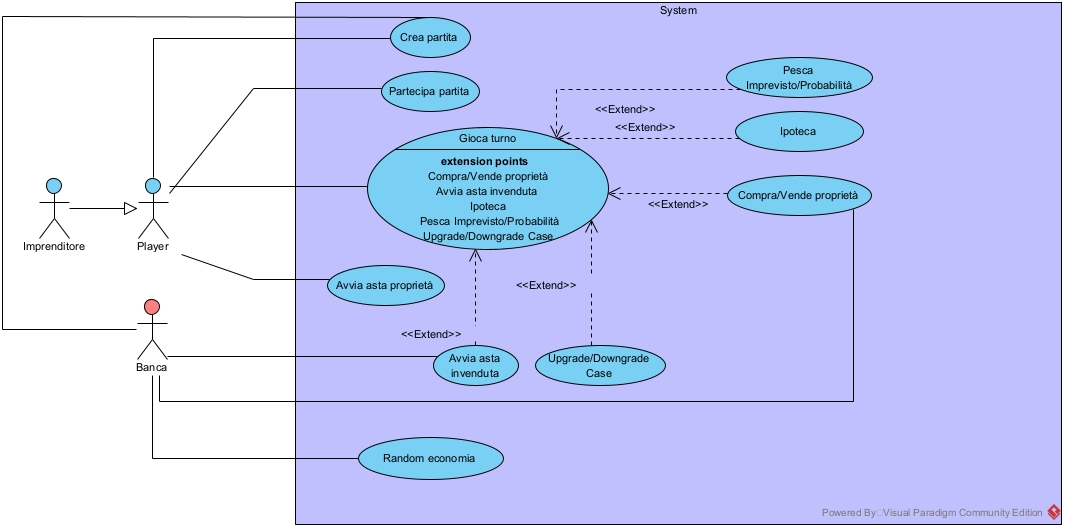
\includegraphics[width=\textwidth]{ModelloCasiDUso}}
	\caption{Diagramma dei Casi d'Uso}
	\end{figure}
	
		\begin{figure}[H]
	\centering
\href{https://github.com/UnimibSoftEngCourse2022/progetto-monopoly-1-gangoffour2/blob/feat/doc/doc/img/ModelloDiDominio.jpg?raw=true}
	{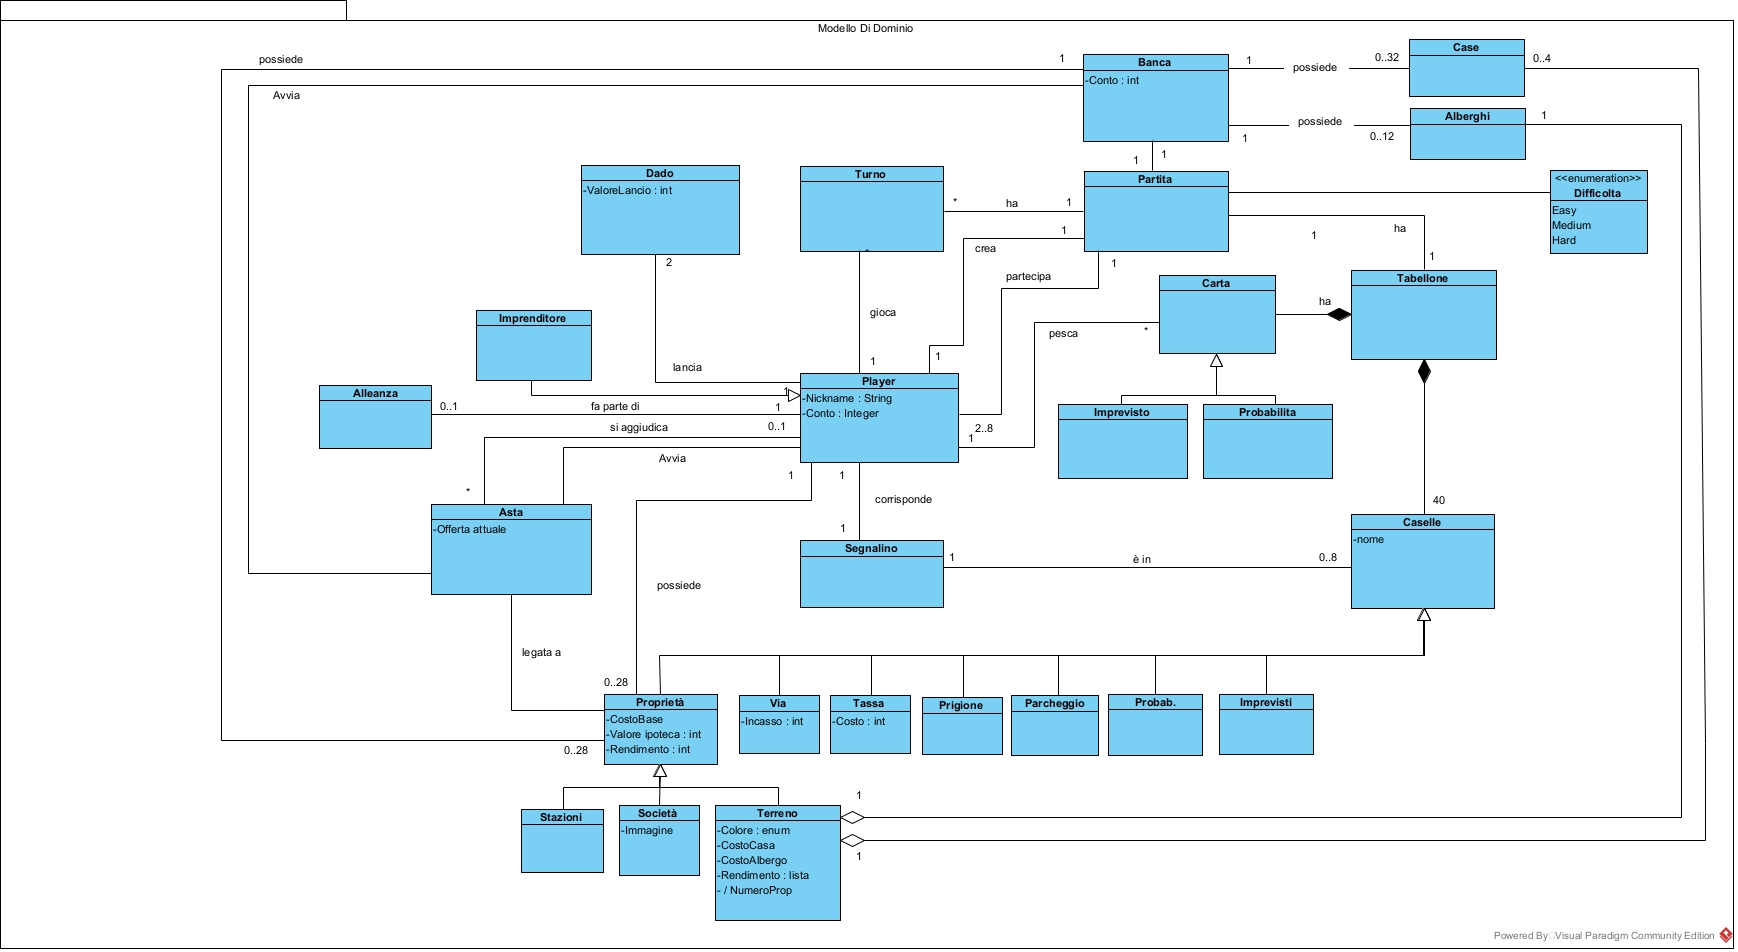
\includegraphics[width=\textwidth]{ModelloDiDominio}}
		\caption{Modello di Dominio}
	\end{figure}

		\begin{figure}[H]
	\centering
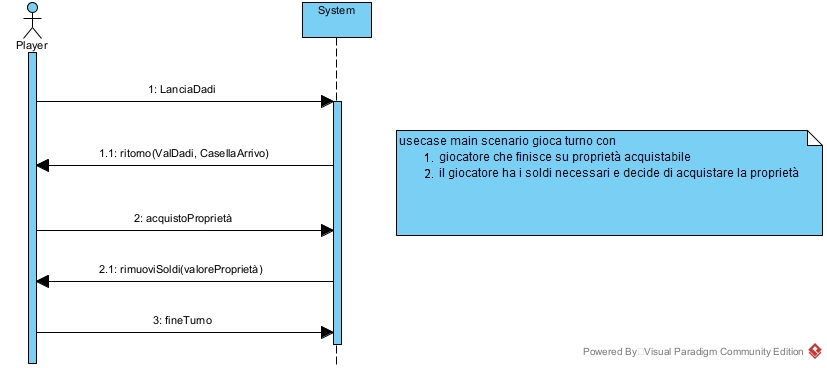
\includegraphics[width=\textwidth]{SSD_GiocaTurno_CasellaProprieta+Acquisto}
		\caption{SSD GiocaTurno CasellaProprieta \& Acquisto}
	\end{figure}
	
	
		\begin{figure}[H]
	\centering
\includegraphics[width=\textwidth]{SSD_GiocaTurno_CasellaProprietà+NoAcquisto}
		\caption{SSD GiocaTurno CasellaProprieta \& No Acquisto}
	\end{figure}


\begin{figure}[H]
\centering
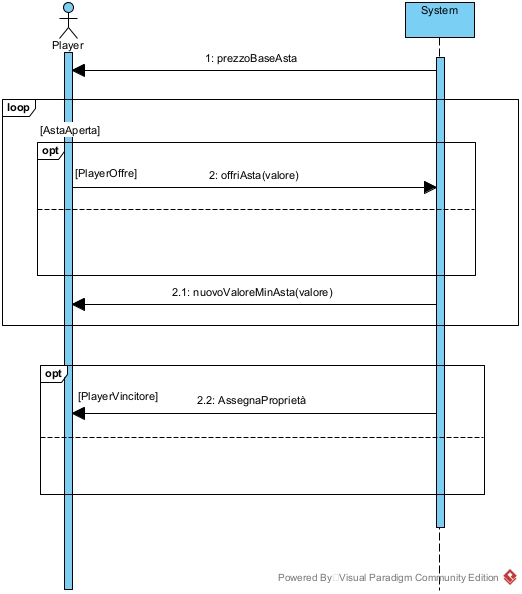
\includegraphics[width=\textwidth]{SSD_IniziaAsta_Invenduta}
\caption{SSD Inizia Asta Terreno invenduto}
\end{figure}


\begin{figure}[H]
\centering
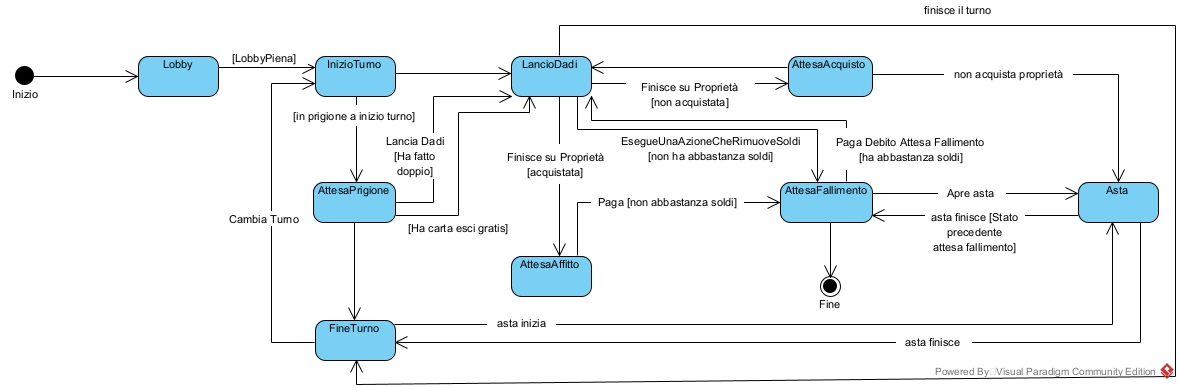
\includegraphics[width=\textwidth]{DiagrammaStatiStatoPartita}
\caption{Diagramma Stati stato partita}
\end{figure}

\begin{figure}[H]
\centering
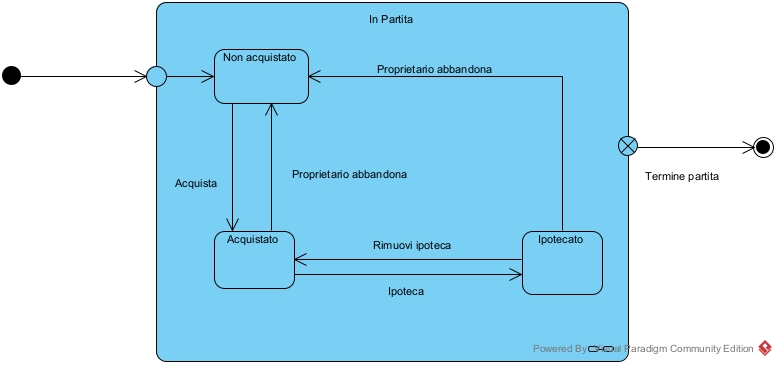
\includegraphics[width=\textwidth]{DiagrammaStatiStatoTerreno}
\caption{Diagramma Stati stato terreno}
\end{figure}

\begin{figure}[H]
\centering
\includegraphics[width=\textwidth]{img/DiagrammaAttivitàEsecuzioneTurno.jpg}
\caption{Diagramma delle Attività - Esecuzione Turno}
\end{figure}



\section{Progettazione}
\subsection{Diagrammi prodotti}
\begin{figure}[H]
\centering
\href{https://github.com/UnimibSoftEngCourse2022/progetto-monopoly-1-gangoffour2/blob/feat/doc/doc/img/DiagrammaDiSequenzaDiProgettazioneTurnoGiocatore.jpg?raw=true}
	{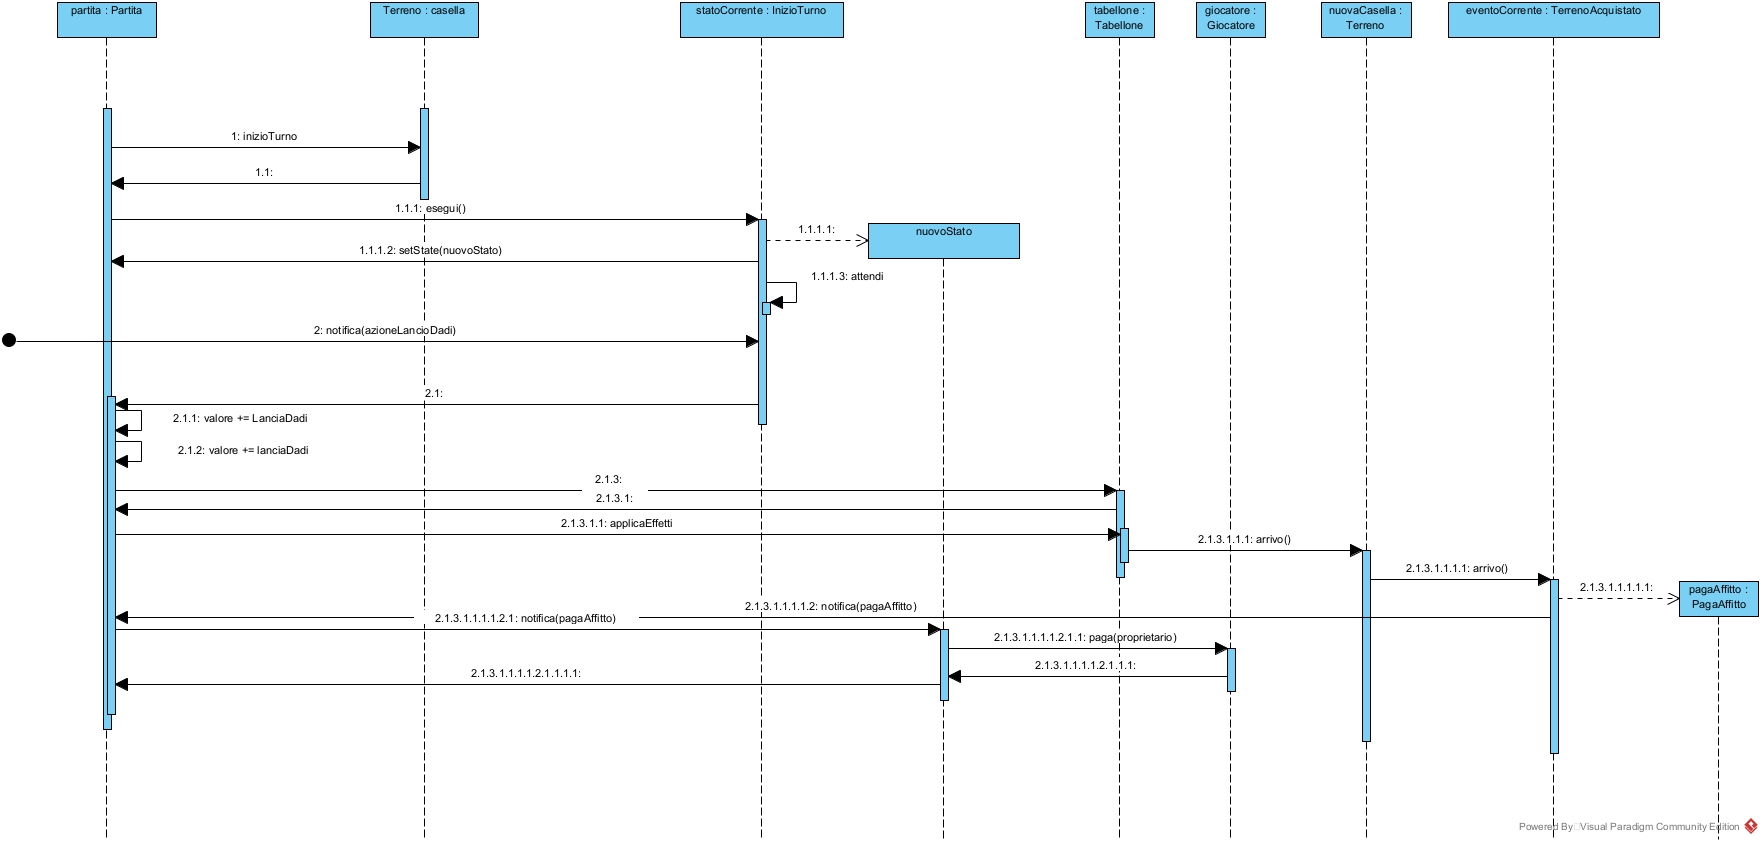
\includegraphics[width=\textwidth]{DiagrammaDiSequenzaDiProgettazioneTurnoGiocatore}}
\caption{Diagramma Stati stato terreno}
\end{figure}

\begin{figure}[H]
\centering
\href{https://github.com/UnimibSoftEngCourse2022/progetto-monopoly-1-gangoffour2/blob/feat/doc/doc/img/DiagrammaDelleClassi.jpg?raw=true}
	{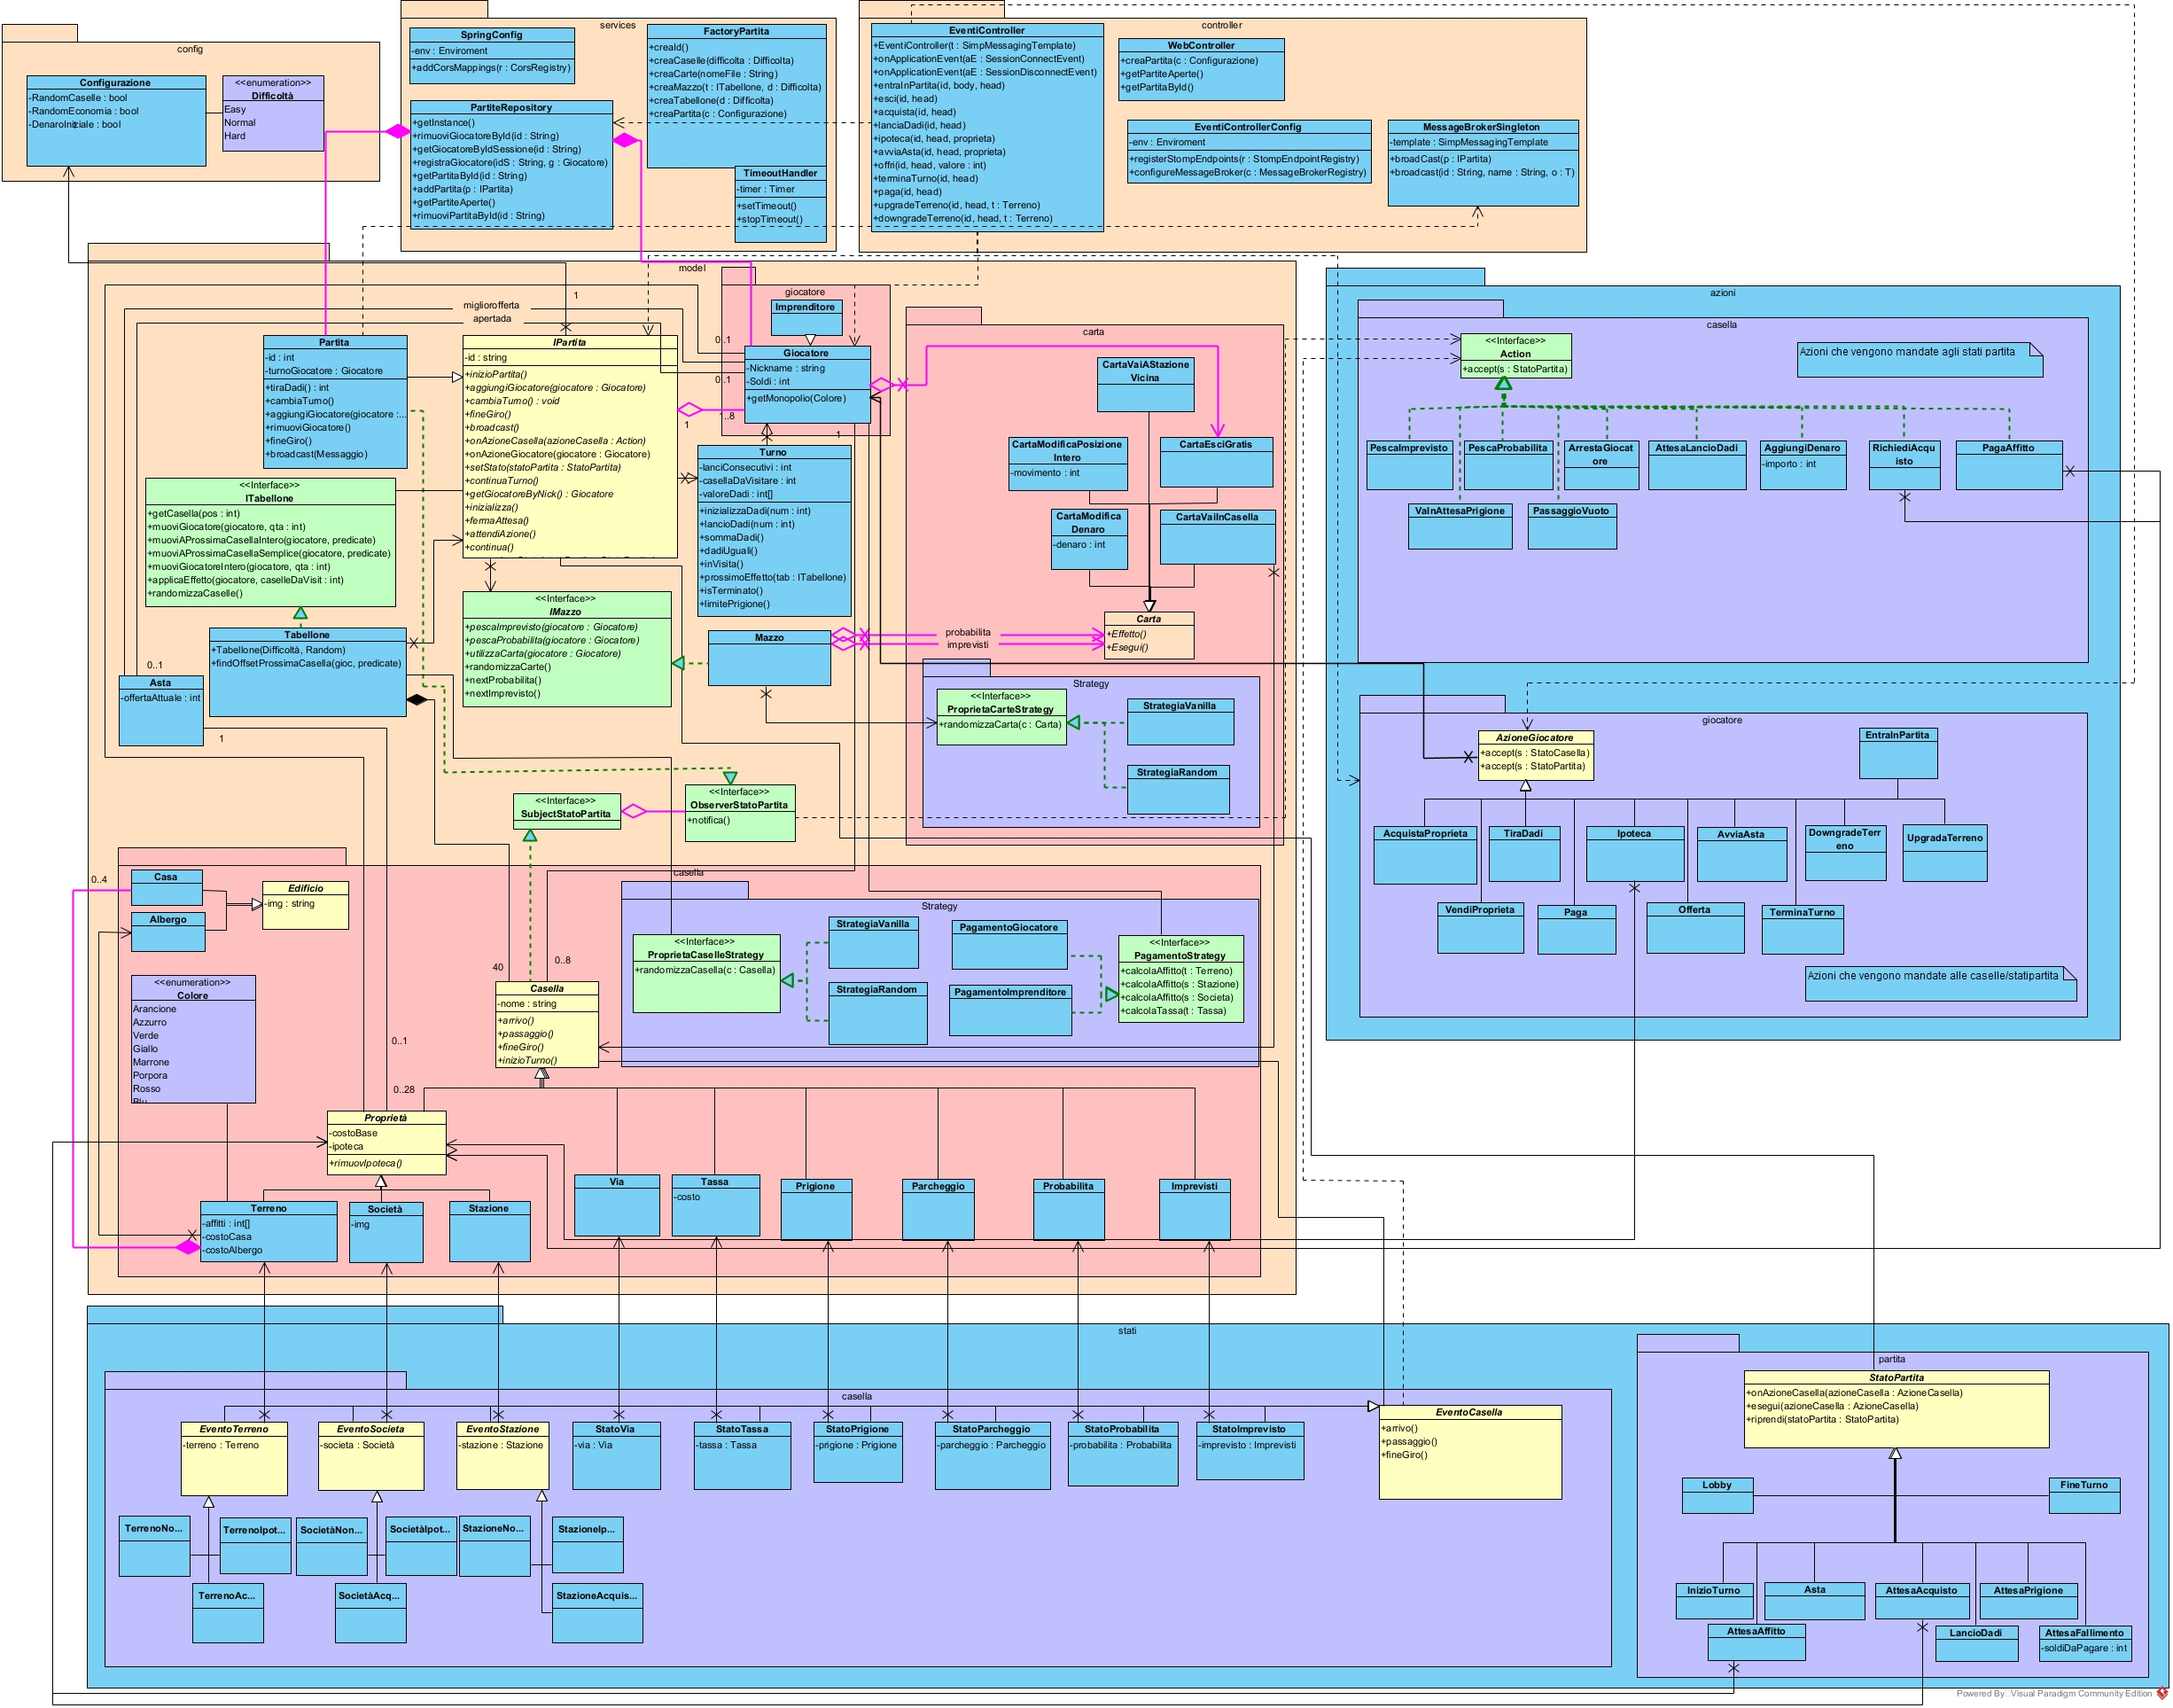
\includegraphics[width=\textwidth]{img/DiagrammaDelleClassi.jpg}}
\caption{Diagramma delle classi di progetto}
\end{figure}

\begin{figure}[H]
\centering
\href{https://github.com/UnimibSoftEngCourse2022/progetto-monopoly-1-gangoffour2/blob/feat/doc/doc/img/Diagramma_Architettura_Software.jpg?raw=true}
	{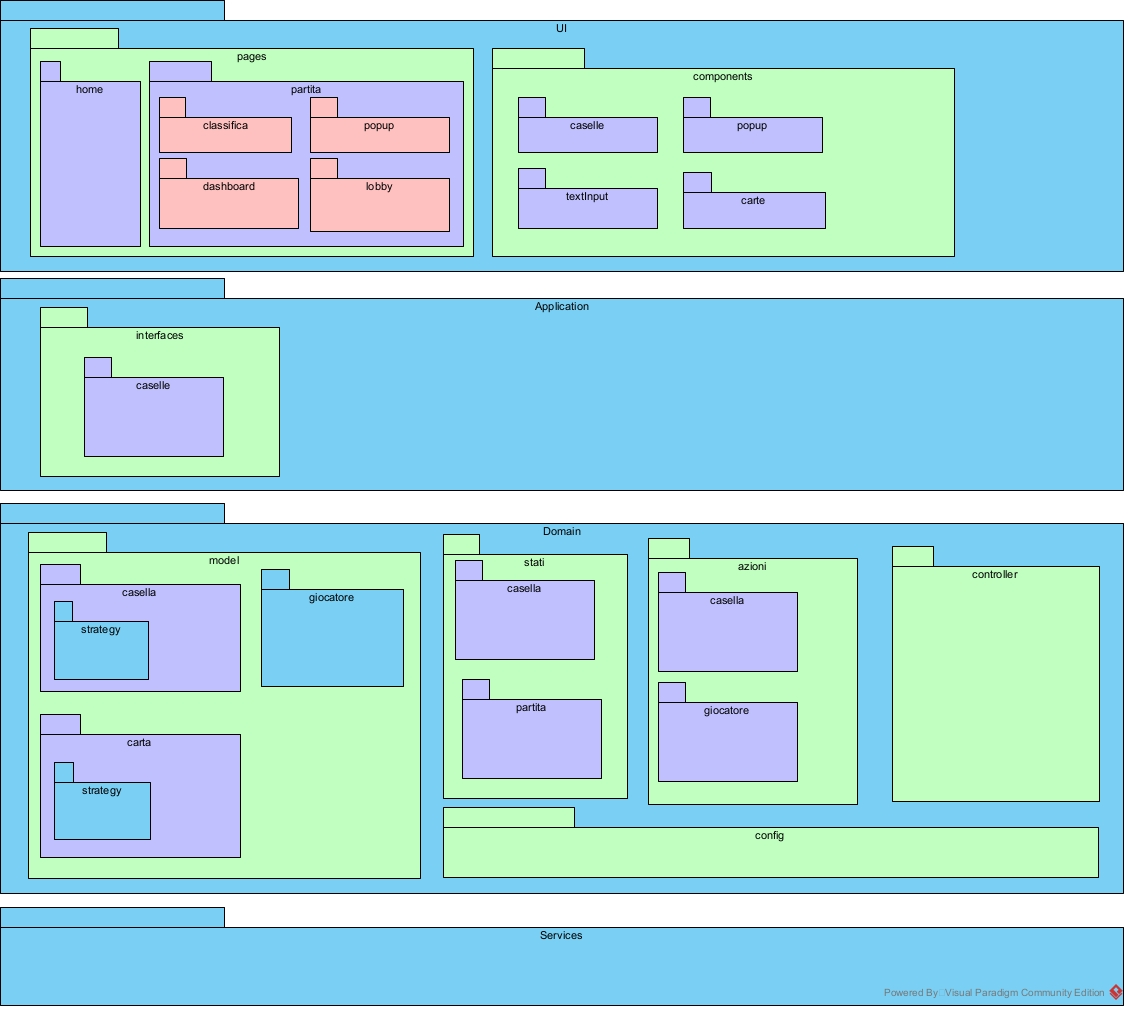
\includegraphics[width=\textwidth]{Diagramma_Architettura_Software}}
\caption{Diagramma Architettura Software}
\end{figure}


\begin{figure}[H]
\centering
\href{https://github.com/UnimibSoftEngCourse2022/progetto-monopoly-1-gangoffour2/blob/feat/doc/doc/img/DiagrammaDiDeployment.jpg?raw=true}
	{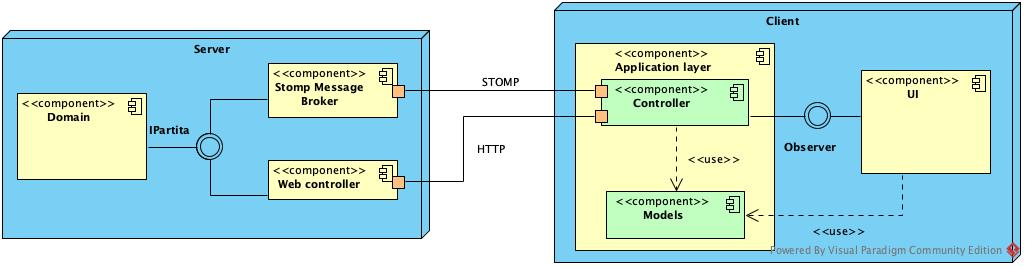
\includegraphics[width=\textwidth]{img/DiagrammaDiDeployment.jpg}}
\caption{Diagramma di deployment}
\end{figure}

Nella progettazione abbiamo usufruito del polimorfismo per fare in modo che le diverse tipologie delle caselle potessero rispondere in modi differenti in base al tipo di azione che ricevevano. \\
Inoltre alcune caselle sono dotate di stati per fare in modo che anche lo stato potesse generare diverse logiche di gestione delle azioni.

\subsection{Tecnologie utilizzate}
\begin{itemize}
	\item \textbf{Server}: per il backend abbiamo voluto utilizzare il framework Spring sia perché complessivamente tutto il team conosce Java e ha avuto esperiente con il framework sia perché ritenuto idoneo allo scopo.


	\item \textbf{Client}: per il frontend è stata principalmente utilizzata la libreria React per costruire l'interfaccia grafica per interagire con il server e costruire dinamicamente il tabellone.
	Sebbene non tutto il team sapesse come utilizzare questa libreria abbiamo convenuto fosse la scelta più ragionevole per l'elevata esperienza di alcuni membri del team che si sono concentrati sullo sviluppo del client.
	
	\item \textbf{Altro}: Sonarqube in locale e Sonarcloud per la CI/CD Pipeline
\end{itemize}


\subsection{Principi SOLID}
Nello sviluppo del progetto siamo stati guidati dai principi \textbf{SOLID}:
\begin{itemize}
    \item \textbf{S}ingle-Responsibility principle: classi come Partita, Tabellone e Turno tendono a gestire specifici aspetti del gioco e ad esempio sono state divise concettualmente le caselle, i loro stati e i loro comportamenti.
    
    \item \textbf{O}pen closed principle: il sistema è stato progettando cercando di lasciare la massima possibilità di estenderlo senza andarne a modificare la struttura: ad esempio, è possibile aggiungere un nuovo stato,una nuova casella o nuovi comportamenti senza modificare la struttura principale del sistema: è sufficiente ridefinire i metodi per gestire determinati eventi senza preoccuparsi di modificare il resto del software.
    
    \item \textbf{L}iskov Substitution Principle: Per fare in modo che la struttura della partita e il suo corretto comportamento non siano influenzati dalla tipologia della singola casella, abbiamo fatto in modo di rendere la gerarchia delle caselle completamente trasparente alla partita.
    
    \item \textbf{I}nterface Segregation Principle: le interfacce utilizzano la keyword default per definire una implementazione base dei metodi che espongono. In questo modo, le classi che implementano tali interfacce sovrascrivono soltanto i metodi che ha effettivamente senso implementare.
    
    \item \textbf{D}ependency Inversion: Per diminuire l'accoppiamento tra classi concrete e aumentare la dipendenza verso classi astratte, abbiamo introdotto varie interfacce che nascondono le implementazioni, tra cui: ITabellone, IPartita, IMazzo.
    \end{itemize}

\subsection{Principi PHAME Utilizzati}
\begin{itemize}
        \item Encapsulation: Abbiamo cercato di fare in modo che ogni classe nascondesse i dettagli di implementazione: ad esempio, Quando un giocatore deve aggiudicarsi una proprietà, viene chiamato un metodo su di esso piuttosto che accedere ai suoi attributi. Questo fa bene anche al Single responsibility principle.
        \item Hierarchy: per cercare di semplificare la logica del gioco, abbiamo creato una gerarchia di caselle, le quali condividono un sottoinsieme di attributi (ad esempio il nome), ma aggiungono o ridefiniscono comportamenti in base al loro tipo. Sfruttando il polimorfismo, È più facile raggiungere un basso livello di disaccoppiamento con il tabellone, che ha bisogno di conoscere solo la radice di questa gerarchia.
    \end{itemize}
    

\subsection{Design patterns utilizzati}
    \begin{itemize}
        \item \textbf{Singleton}: utile per salvare informazioni a cui si può accedere da ogni parte del programma ottenendo sempre la stessa istanza. 
        
        
        \textit{Classi interessate: MessageBrokerSingleton, FactoryPartita, PartiteRepository} 
        
        
        \item \textbf{State}: fondamentale nella struttura del progetto. È stato utilizzato perché il comportamento all'interno di una partita dipende dallo stato di ogni casella, in combinazione con lo stato della partita. Ad esempio, la terminazione su un terreno deve rispondere in modo diverso in base a se è stato acquistato, ipotecato, ecc… \\ La stessa cosa vale per la partita: se la partita sta attendendo che un giocatore paghi l'affitto per un terreno, non è possibile che un altro giocatore lanci i dadi in quel momento. 
        
        \textit{Classi interessate: StatoPartita, StatoCasella, Partita, Casella} 
        
        
        \item \textbf{Visitor}: Quando una casella notifica un'azione da eseguire alla partita (o meglio, al suo stato), il metodo da eseguire dipende dal tipo concreto di questa azione. \\Per esempio, dato uno stato, il comportamento dipende dal tipo dell'azione generata dalla casella. Inoltre, in questo modo, è possibile aggiungere nuove azioni senza dover modificare la struttura delle classi.\\Tramite la tecnica del Double dispatch è stato possibile eseguire azioni differenti che differiscono per il tipo di azione generata dalle caselle. L'effetto di questo pattern è la "Creazione" di un automa a stati le cui transizioni dipendono dalle coppie stato corrente/azione
        
        \textit{Classi interessate: AzioniGiocatore, AzioniPartita} 
        
        
        \item \textbf{Strategy}: Utilizzati rispettivamente per per la gestione della randomizzazione di Caselle sul tabellone, di costi delle caselle, di attributi delle carte e definizione di comportamenti diversi per un giocatore di tipo Imprenditore rispetto a uno Standard. 
        \\Il mazzo di carte e il tabellone hanno uno strategy istanziato durante la creazione della partita in base alla difficoltà selezionata. Quando necessario, viene chiamato un metodo su quello strategy che conterrà la logica di gestione specifica per quella difficoltà.
        \\Tutto questo sempre seguendo il principio di apertura ai cambiamenti che in questo permetterà facilmente estendere il software a diversi tipi di strategie legate alle difficoltà di gioco.
        
         \textit{Classi interessate: (Interfaccia)PagamentoStrategy, PagamentoStrategiaGiocatore, PagamentoStrategiaImprenditore, (Interfaccia)ProprietaCaselleStrategy, StrategiaCasellaRandom, StrategiaCasellaVanilla, (Interfaccia)ProprietaCarteStrategy, StrategiaCarteRandom, StrategiaCarteVanilla}
         
         
         \item \textbf{Facade}: La partita agisce da Facade intercettando tutte le richieste dei controller. \\
         \textit{Classi interessate: IPartita}
         
         
         \item \textbf{Observer}: Usato nel client per far intercettare l’aggiornamento della partita da più componenti contemporaneamente e nel server per evitare le dipendenze cicliche nelle comunicazioni tra partita e casella e viceversa
         
         \textit{Classi interessate clienti: ObserverCarte, ObserverPartite, ObserverSingleton}
         \textit{Classi interessate server: ObserverStatoPartita, SubjectStatoPartita}

         \item \textbf{Builder}: Usato tramite libreria Lombok di Maven evita di utilizzare costruttori esplicitamente e errori di coerenza nell'istanziazione degli oggetti.
         
         \textit{Classi interessate server: Tutte}
         
    \end{itemize}

\subsection{Pattern architetturali utilizzati}
    \begin{itemize}
        \item \textbf{Front controller}: utile per fornire un punto di accesso al backend dal client. Classi interessate: EventiController, WebController.
        \item \textbf{Message channel}: utilizzato per gestire le sessioni delle partite con i client. Per fare in modo che tutti i giocatori ricevessero lo stato della partita aggiornato, abbiamo utilizzato un message broker al quale si iscrivono.
        \item \textbf{Layers}: il suo utilizzo ci ha consentito di organizzare l’architettura logica in un sistema di più livelli (layers) con funzionalità distinte ma correlate. In modo tale da avere una separazione delle responsabilità pulita e che aumenti la coesione del sistema finale.
    \end{itemize}
    



\subsection{Problemi incontrati durante la fase di progettazione}
\paragraph{Antipattern strutturali}
Utilizzando il tool Understand, abbiamo notato che la classe Partita aveva molte dipendenze in ingresso e in uscita: questo può essere segno di un antipattern Hub. Per cercare di risolvere il problema, abbiamo aggiunto una classe astratta che viene estesa da partita: In questo modo, abbiamo ridotto le dipendenze in entrata da partita, rendendo visibile solo la classe astratta relativa. Stessa cosa per ITabellone.
\\Invece StatoPartita ha molte dipendenze in entrata, una per ogni tipo di azione 
giocatore/casella. Questo implica che ci potremmo trovare davanti a un Global Butterfly.

\end{document}